\documentclass[12pt]{article}
\usepackage{enumerate}
\usepackage{notes}
\usepackage{oxford}

\begin{document}
\title{Oxford A0 - Linear Algebra \footnotetext{\url{https://courses.maths.ox.ac.uk/node/5353}}}
\author{Dan Davison}
\maketitle

\section*{Sheet 1}

\subsection*{} % 1
\begin{mdframed}
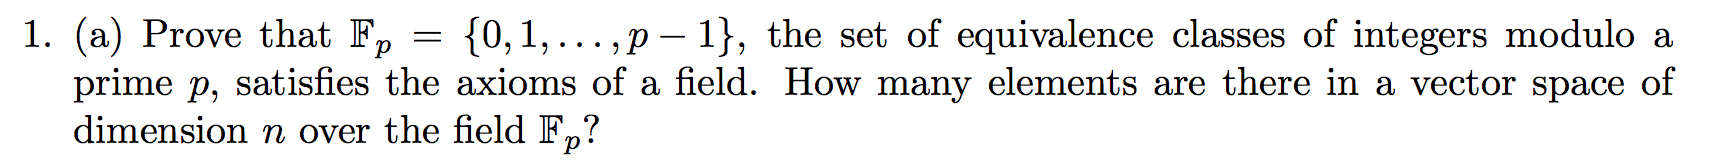
\includegraphics[width=450pt]{img/linear-algebra-a0-1-1-a.png}\\
\end{mdframed}

Let\footnote{Unlike the question, I am trying to use notation that
  distinguishes between integers and their equivalence classes.}
$a, b, c \in \Z$ with $0 \leq a < p, ~~ 0 \leq b < p, ~~ 0 \leq c < p$.

Let $\bar a, \bar b, \bar c \in \F$ be equivalence classes of integers modulo $p$.

The field axioms are listed below, together with proof that they hold for $\F_p$.
\begin{enumerate}
\item \textbf{$\F_p$ is an abelian group under addition}\\
  Define $\bar a + \bar b := \bar{a + b}$, then:
  \begin{enumerate}
  \item \textit{Existence of identity}: $\bar 0$ is the identity since
    $\bar a + \bar 0 = \bar{a + 0} = \bar{a}$ for all $\bar a \in \F_p$.
  \item \textit{Existence of inverses}: $(\bar a)^\1 = \bar{-a}$ since
    $\bar a + \bar{-a} = \bar{a + -a} = \bar{0}$ for all $a \in \F_p$.
  \item \textit{Commutativity}:
    $\bar a + \bar b = \bar{a + b} = \bar{b} + \bar{a}$ for all $a, b \in \F_p$.
  \item \textit{Associativity}:
    $\bar a + (\bar b + \bar c) = \bar a + \bar {b + c} = \bar{a + b + c} =
    \bar{a + b} + \bar{c} = (\bar a + \bar b) + \bar{c}$.
  \end{enumerate}
\item \textbf{$\F_p\setminus\{\bar 0\}$ is an abelian group under multiplication}\\
  Define $\bar a ~ \bar b := \bar{ab}$, then:
  \begin{enumerate}
  \item \textit{Existence of identity}: $\bar 1$ is the identity since
    $\bar a \bar 1 = \bar{a\cdot 1} = \bar{a}$ for all $\bar a \in \F_p$.
    \newpage
  \item \textit{Existence of inverses for everything except additive identity}:\\\\
    The claim is that for all $\bar a \in \F_p \setminus \{\bar 0\}$ there
    exists $\bar b \in \F_p$ such that $\bar a ~ \bar b = \bar 1$.

    \textbf{Proof 1}\\
    We show that elements cannot repeat in a row/column of the group operation
    table, therefore something muct be the inverse.
    \begin{align*}
      a \cdot b &= a \cdot c \mod p\\
      a(b - c) &= 0 \mod p\\
      a &= 0 \text{~or~~} b = c \mod p
    \end{align*}

    \textbf{Proof 2}\\
    Fix an arbitrary $a \in \{1, \ldots, p-1\}$.

    The claim is equivalent to the following: there exists
    $b \in \{0, 1, \ldots, p\}$ such that for all $i, j \in \Z$ there exists
    $k \in \Z$ such that $(ip + a)(jp + b) = kp + 1$.

    But note that $(ip + a)(jp + b) = p(ijp + aj + bi) + ab$ and therefore
    \begin{align*}
      &(ip + a)(jp + b) = kp + 1\\
      \iff &ab = p(k - ijp - aj - bi) + 1.
    \end{align*}
    Since $k$ can be chosen freely, the condition is simply that for all
    $i, j \in \Z$ there exists $k \in \Z$ such that $ab = kp + 1$.

    Note\footnote{I eventually allowed myself to google for a hint here which
      brought up people pointing to Bezout's identity.} that $a$ and $p$ are
    coprime (gcd is 1). By Bezout's identity, there exists $b, -k \in \Z$
    such that
    \begin{align*}
      ba + (-k)p = 1 \iff ab = kp + 1. \qed
    \end{align*}


  \item \textit{Commutativity}:
    $\bar a ~ \bar b = \bar{ab} = \bar{b} ~ \bar{a}$ for all $a, b \in \F_p$.
  \item \textit{Associativity}:
    $\bar a (\bar b \bar c) = \bar a + \bar {bc} = \bar{abc} =
    \bar{ab}~\bar{c} = (\bar a ~ \bar b) \bar{c}$.
  \end{enumerate}
\item \textbf{Distributive axiom}
  \begin{enumerate}
  \item \textit{Multiplication distributes over addition}: $\bar a (\bar b + \bar c) = \bar a (\bar{b + c}) = \bar{a(b+c)} = \bar{ab +
    ac} = \bar{ab} + \bar{ac} = \bar{a}~\bar{b} + \bar{a}~\bar{c}$
  \end{enumerate}
\end{enumerate}

There are $p^n$ elements in a vector space of dimension $n$ over the field $\F_p$.
\newpage
\begin{mdframed}
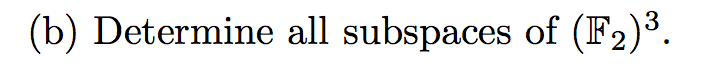
\includegraphics[width=200pt]{img/linear-algebra-a0-1-1-b.png}
\end{mdframed}

\textit{Remark}: This is like the 8 vectors that form the unit cube in
$\R^3$, except that when extended beyond the cube by vector addition or
scalar multiplication they ``wrap around''.

Note that
\begin{align*}
  (\F_2)^3 = \{&\bar 0, \bar 1\}^3\\
           = \{&(\bar 0, \bar 0, \bar 0),\\
               &(\bar 0, \bar 0, \bar 1),\\
               &(\bar 0, \bar 1, \bar 0),\\
               &(\bar 0, \bar 1, \bar 1),\\
               &(\bar 1, \bar 0, \bar 0),\\
               &(\bar 1, \bar 0, \bar 1),\\
               &(\bar 1, \bar 1, \bar 0),\\
               &(\bar 1, \bar 1, \bar 1)\}.
\end{align*}
The set of subspaces of $(\F_2)^3$ is
\begin{align*}
  &\{\{(\bar 0, \bar 0, \bar 0)\}\} ~~~~~~~~~~~~~~~~~~~~~ \cup\\
  &\{\{(\bar 0, \bar 0, \bar 0), x\} ~|~ x \in (\F_2)^3\} ~~~ \cup\\
  &\{\{(\bar 0, a, b) ~|~ a, b \in \F_2\}\}  ~~~~~~~ \cup\\
  &\{\{(a, \bar 0, b) ~|~ a, b \in \F_2\}\}  ~~~~~~~ \cup\\
  &\{\{(a, b, \bar 0) ~|~ a, b \in \F_2\}\}  ~~~~~~~ \cup\\
  &\{(\F_2)^3\}.
\end{align*}

\red{Per AC this is missing, at least, a subspace of size 4. Also see Sylov theorems.}

\newpage
\subsection*{} % 2
\begin{mdframed}
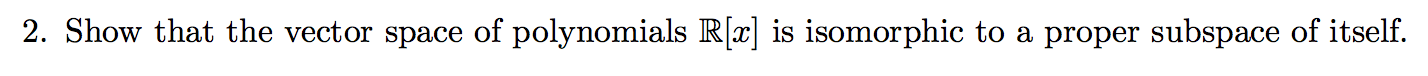
\includegraphics[width=450pt]{img/linear-algebra-a0-1-2.png}\\
\end{mdframed}
We need to:
\begin{enumerate}
\item \textbf{Exhibit a proper subspace $S[x] \subset \R[x]$ and a bijection $f:\R[x] \to S[x]$}\\\\
  Let $a_i \in \R$ for $i = 0, 1, 2, \ldots$ so that
  $\R[x] = \{a_0 + a_1x^1 + a_2x^2 + \ldots\}$.

  Define $S[x] = \{0 + a_1x^1 + a_2x^2 + a_3x^3 + \ldots\}$, i.e. the restriction
  of $\R[x]$ to those polynomials that have constant term zero.

  $S[x]$ is a proper subspace of $\R[x]$ since it contains the zero polynomial,
  and is closed under addition and scalar multiplication.

  Define $f: \R[x] \to S[x]$ where
  $f(a_0 + a_1x^1 + a_2x^2 + \ldots) = 0 + a_0x^1 + a_1x^2 + a_2x^3 + \ldots$.

  $f$ is clearly injective, since if $f(r(x)) = f(r'(x))$ then their
  coefficients $a_0, a_1, \ldots$ are the same and hence $r(x) = r'(x)$.

  Also, $f$ is clearly surjective since if
  $s(x) = a_1x^1 + a_2x^2 + a_3x^3 + \ldots$ then
  $s(x) = f(a_1 + a_2x^1 + a_3x^2 + \ldots)$.

\item \textbf{Prove that $f$ preserves addition}\\\\
  Let $a_i,b_i \in \R$ for $i = 0, 1, 2, \ldots$

  Let $r(x) = a_0 + a_1x^1 + a_2x^2 + \ldots$ and $r'(x) = b_0 + b_1x^1 + b_2x^2 + \ldots$.

  Then
  \begin{align*}
    f\Big(r(x) + r'(x)\Big)
    &= f\Big((a_0 + b_0) + (a_1 + b_1)x^1 + (a_2 + b_2)x^2 + \ldots\Big)\\
    &= 0 + (a_0 + b_0)x^1 + (a_1 + b_1)x^2 + (a_2 + b_2)x^3 + \ldots\\
    &= \Big(0 + a_0x^1 + a_1x^2 + a_2x^3 + \ldots \Big) \\
    &+ \Big(0 + b_0x^1 + b_1x^2 + b_2x^3 + \ldots \Big) \\
    &= f\Big(r(x)\Big) + f\Big(r'(x)\Big).
  \end{align*}

  \begin{align*}
  \end{align*}

\item \textbf{Prove that $f$ preserves scalar multiplication}
  \begin{align*}
    f\Big(\lambda r(x)\Big)
    &= f\Big(\lambda a_0 + \lambda a_1x^1 + \lambda a_2x^2 + \ldots \Big) \\
    &= 0 + \lambda a_0x^1 + \lambda a_1x^2 + \lambda a_2x^3 + \ldots \\
    &= \lambda(0 + a_0x^1 + a_1x^2 + a_2x^3 + \ldots) \\
    &= \lambda f\Big(r(x)\Big)
  \end{align*}


\end{enumerate}

\newpage
\subsection*{} % 3
\begin{mdframed}
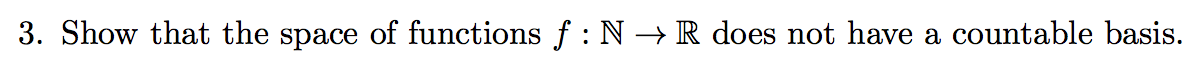
\includegraphics[width=400pt]{img/linear-algebra-a0-1-3.png}\\
\end{mdframed}

Note:
\begin{enumerate}
\item The space of functions $f:\N \to \R$ is the space of real-valued
infinite sequences.
\item A basis is countable iff a bijection exists between the basis and $\N$.
\end{enumerate}

\red{I haven't managed to do this. What follows is what I was thinking, but
  must be wrong since it contradicts the question.}

Let $x_i \in \R$ for
$i \in \N$ and define the following:
\begin{itemize}
\item $F_n := \{(x_1, x_2, \ldots, x_n) ~|~ x_1, x_2, \ldots, x_n \in \R\}$ is
  the space of functions\\$f:\{1,2, \ldots, n\} \to \R$
\item $F_\infty := \{(x_1, x_2, \ldots) ~|~ x_1, x_2, \ldots \in \R\}$ is the
  space of functions $f:\N \to \R$.
\end{itemize}

Note that $F_1 = \{x_1 ~|~ x_1 \in \R\} = \R$. Therefore every basis for $F_1$ has cardinality
1 (every basis is a set containing a single non-zero real number).

Similarly, $F_2 = \R^2$, and every basis of $F_2$ has cardinality 2.

\red{Basically it seems like the following is a basis of this space of functions,
but it is countable:}
\begin{align*}
  &(1, 0, 0, \ldots),\\
  &(0, 1, 0, \ldots),\\
  &(0, 0, 1, \ldots),\\
  &\ldots\\
\end{align*}

\red{I think the answer here is that $E$ is a basis for $F_\infty$ iff every
  element of $F_\infty$ can be expressed as a linear combination of a
  \textit{finite} number of elements from $E$. But this is untrue, at least for
  the basis I have suggested, since for example the constant function
  $f(i) = 1 ~\forall i$ fails.}

% ~\\
% \hrule




\newpage
\subsection*{} % 4
\begin{mdframed}
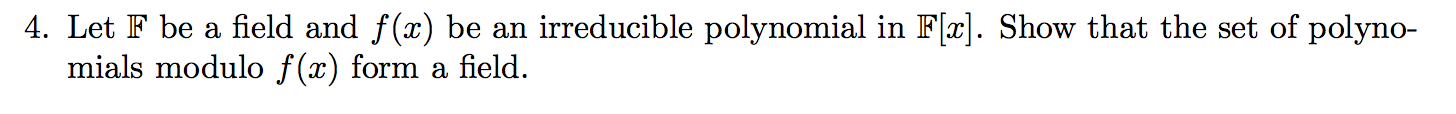
\includegraphics[width=400pt]{img/linear-algebra-a0-1-4.png}\\
\end{mdframed}
Let $P$ be the set of polynomials modulo $f(x)$.

The field axioms are listed below, together with proof that they hold for $P$.
\begin{enumerate}
\item \textbf{$P$ is an abelian group under addition}\\\\
  Define $\bar{g(x)} + \bar{h(x)} := \bar{g(x) + h(x)}$, then:
  \begin{enumerate}
  \item \textit{Existence of identity}:\\
    The additive identity is $\bar 0 = \Big\{f(x)g(x) ~|~ g(x) \in \F[x]\Big\}$.

  \item \textit{Existence of inverses}:\\
    $\bar{g(x)}^{~\1} = \bar{-g(x)}$ for all $g(x) \in P$.
  \item \textit{Commutativity and Associativity}:\\
    Proofs of these are essentially the same as for $\F_p$ (question 1).
  \end{enumerate}
\item \textbf{$P\setminus\{\bar 0\}$ is an abelian group under multiplication}\\\\
  Define $\bar{g(x)} \cdot \bar{h(x)} := \bar{g(x)\cdot h(x)}$, then:
  \begin{enumerate}
  \item \textit{Existence of identity}:\\
    The multiplicative identity is $\bar 1 = \Big\{f(x)g(x) + 1~|~ g(x) \in \F[x]\Big\}$.

  \item \textit{Existence of inverses for everything except additive identity}:\\\\
    The claim is that for all $\bar a \in \F_p \setminus \{\bar 0\}$ there
    exists $\bar b \in \F_p$ such that $\bar a ~ \bar b = \bar 1$.

    Fix an arbitrary $a \in \{1, \ldots, p-1\}$.

    The claim is equivalent to the following: there exists
    $b \in \{0, 1, \ldots, p\}$ such that for all $i, j \in \Z$ there exists
    $k \in \Z$ such that $(ip + a)(jp + b) = kp + 1$.

    But note that $(ip + a)(jp + b) = p(ijp + aj + bi) + ab$ and therefore
    \begin{align*}
      &(ip + a)(jp + b) = kp + 1\\
      \iff &ab = p(k - ijp - aj - bi) + 1.
    \end{align*}
    Since $k$ can be chosen freely, the condition is simply that for all
    $i, j \in \Z$ there exists $k \in \Z$ such that $ab = kp + 1$.

    Note\footnote{I eventually allowed myself to google for a hint here which
      brought up people pointing to Bezout's identity.} that $a$ and $p$ are
    coprime (gcd is 1). By Bezout's identity, there exists $b, -k \in \Z$
    such that
    \begin{align*}
      ba + (-k)p = 1 \iff ab = kp + 1. \qed
    \end{align*}


  \item \textit{Commutativity}:
    $\bar a ~ \bar b = \bar{ab} = \bar{b} ~ \bar{a}$ for all $a, b \in \F_p$.
  \item \textit{Associativity}:
    $\bar a (\bar b \bar c) = \bar a + \bar {bc} = \bar{abc} =
    \bar{ab}~\bar{c} = (\bar a ~ \bar b) \bar{c}$.
  \end{enumerate}
\item \textbf{Distributive axiom}
  \begin{enumerate}
  \item \textit{Multiplication distributes over addition}: $\bar a (\bar b + \bar c) = \bar a (\bar{b + c}) = \bar{a(b+c)} = \bar{ab +
    ac} = \bar{ab} + \bar{ac} = \bar{a}~\bar{b} + \bar{a}~\bar{c}$
  \end{enumerate}
\end{enumerate}

\newpage

\begin{mdframed}
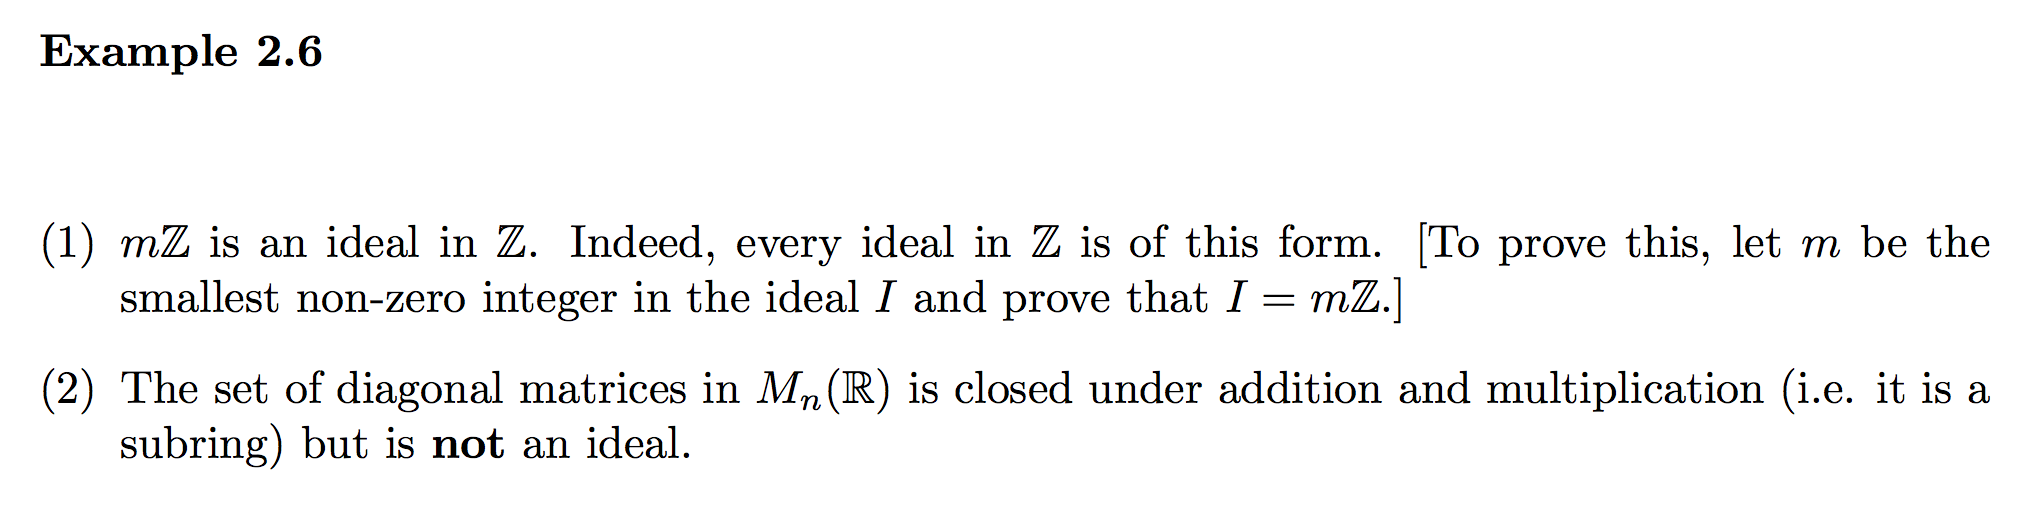
\includegraphics[width=400pt]{img/linear-algebra-eg-2-6.png}
\end{mdframed}

\begin{claim*}
  $m\Z$ is an ideal in $\Z$.
\end{claim*}

\begin{proof}Let $s, t \in m\Z$ and $i, j, k \in \Z$.

  Then $s = mi$ and $t = mj$ for some $i, j$.

  Therefore $s - t = m(i - j) \in m\Z$ and $ks = sk = m(ki) \in m\Z$.
\end{proof}

\begin{claim*}
  Every ideal in $\Z$ is of the form $m\Z$.
\end{claim*}

\begin{proof}
  Let $I$ be an ideal in $\Z$ and let $m$ be the smallest non-zero positive integer in $I$.

  % Let $i \in I$. We have that $i - m \in I$ and that $mi \in I$.

  % We want to show that $i \in m\Z$.

  Let $i \in I$. We want to show that $i \in m\Z$.

  We have:

  $ki \in I$ for all $k \in \Z$.

  $i - j \in I$ for all $j \in I$.

  $i - m \in I$.


 % By the definition of an ideal, $ki \in I$ for
 %  all $k \in \Z$. Therefore $i$ is a multiple of $m$.

  % Conversely, suppose $i \in m\Z$. We want to show that $i \in I$.


  % is a multiple of $m$. So $i = km$ for some $k \in \Z$.
\end{proof}


\newpage
\subsection*{} % 5
\begin{mdframed}
  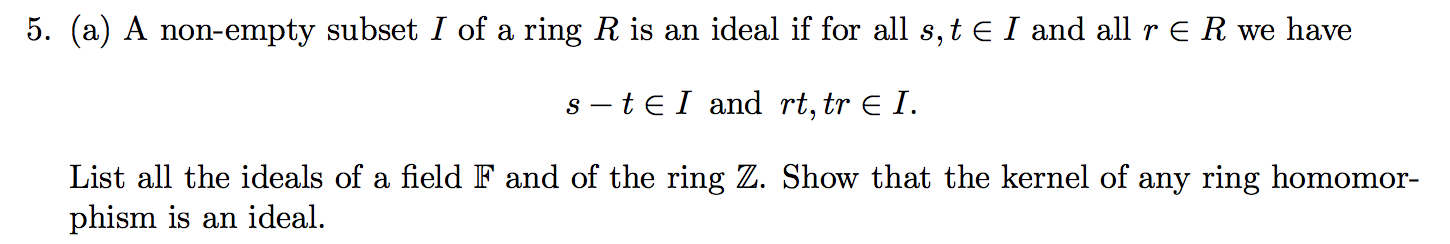
\includegraphics[width=400pt]{img/linear-algebra-a0-1-5-a.png}\\
\end{mdframed}

The set of ideals of a field $\F$ is $\{a\F ~|~ a \in \F\} = \{\{0\}, \F\}$.

The set of ideals of the ring $\Z$ is $\{m\Z ~|~ m \in \Z\}$.


\begin{definition*}
  Let $R, S$ be rings and let $r_1, r_2 \in R$. A \emph{ring homomorphism} is $f:R \to S$ such that
  $f(r_1 + r_2) = f(r_1) + f(r_2)$ and $f(r_1r_2) = f(r_1)f(r_2)$.
\end{definition*}

\begin{claim*}
  The kernel of any ring homomorphism is an ideal.
\end{claim*}

\begin{proof}
  Let $H$ be the kernel of a ring homomorphism $f:R \to S$, and let

  We want to show that
  \begin{enumerate}
  \item $h_1 - h_2 \in H$ for all $h_1, h_2 \in H$, and \label{ring-hom-ideal-1}
  \item $rh \in H$ for all $r \in R, h \in H$. \label{ring-hom-ideal-2}
  \end{enumerate}

  We have $f(h_1 - h_2) = f(h_1) + f(-h_2) = f(h_1) - f(h_2) = 0 - 0 = 0$, proving
  (\ref{ring-hom-ideal-1}).

  And $f(rh) = f(r)f(h) = f(r)\cdot 0 = 0$, proving (\ref{ring-hom-ideal-2}).

\end{proof}



\newpage
\begin{mdframed}
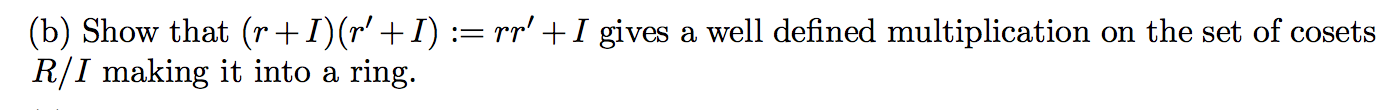
\includegraphics[width=400pt]{img/linear-algebra-a0-1-5-b.png}\\
\end{mdframed}

\begin{mdframed}
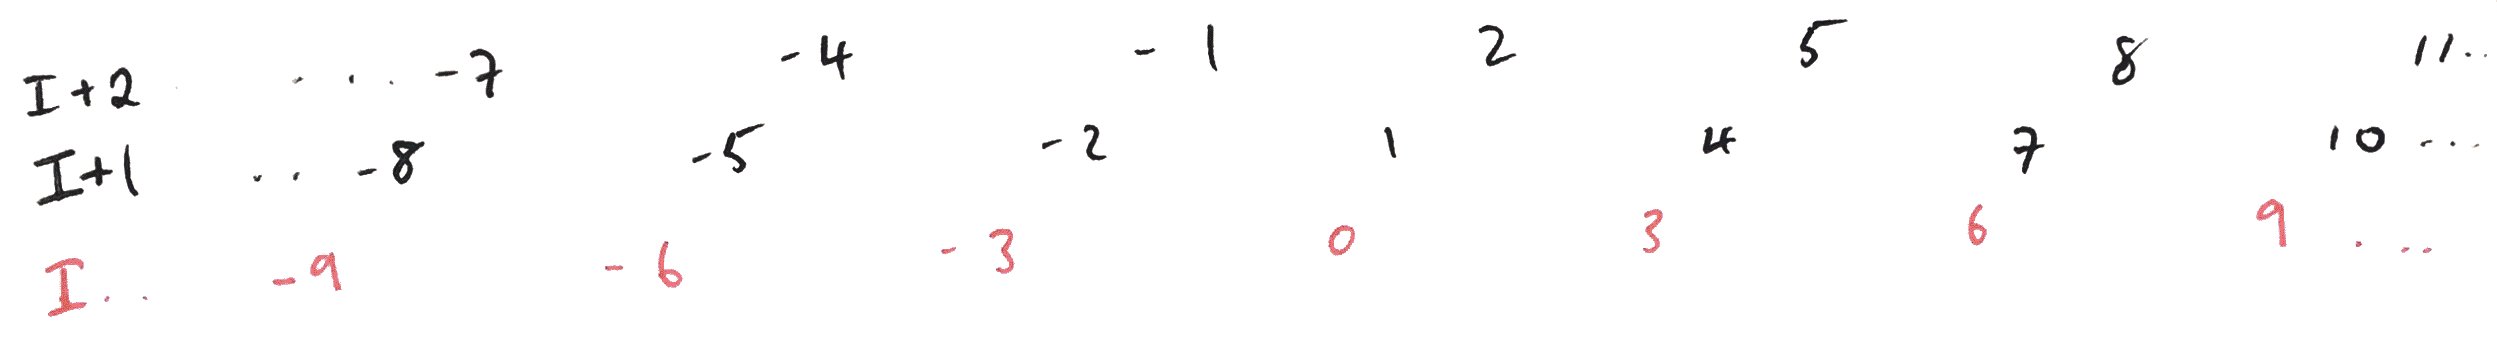
\includegraphics[width=400pt]{img/ideal-in-integers.png}
\end{mdframed}

\begin{mdframed}
\begin{remark*}
  Recall that in group theory a quotient group is formed by:
  \begin{enumerate}
  \item Identify a subgroup.
  \item Form cosets.
  \item Inherit operation on cosets from operation on original group elements.
  \end{enumerate}
  But only if the subgroup is normal.

  Here, the ideal $I$ is playing the role of subgroup.~\\
\end{remark*}
\end{mdframed}

Let $S$ and $T$ be cosets, and let $r \in S$ and $r' \in T$. We need to show that $rr' + I$ is the
same coset, for all choices of $r$, $r'$.

\newpage
\begin{mdframed}
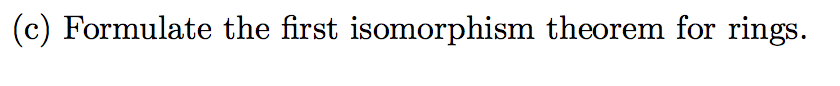
\includegraphics[width=280pt]{img/linear-algebra-a0-1-5-c.png}\\
\end{mdframed}

\newpage
\subsection*{} % 6
\begin{mdframed}
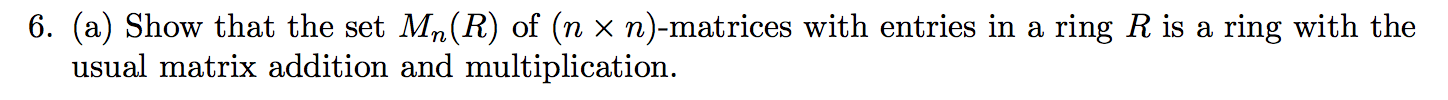
\includegraphics[width=400pt]{img/linear-algebra-a0-1-6-a.png}\\
\end{mdframed}
It is an abelian group under addition since:
\begin{enumerate}
\item The zero matrix is the additive identity.
\item Multiplying a matrix by $-1$ gives its additive inverse.
\item It is closed (result is a matrix of same dimension).
\item Addition commutes.
\end{enumerate}

Under multiplication:
\begin{enumerate}
\item It is closed.
\item Multiplication is associative.
\item Both distributive laws hold ($A(B + C) = AB + AC$ and $(B + C)A = BA + CA$.)
\end{enumerate}

Therefore it is a ring (but not a field since multiplicative inverses may not exist).

\begin{mdframed}
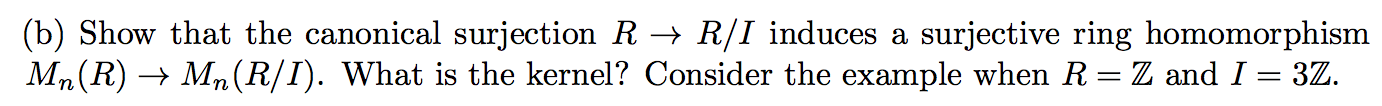
\includegraphics[width=400pt]{img/linear-algebra-a0-1-6-b.png}\\
\end{mdframed}
Let $I$ be an ideal of a ring $R$.

Note that:
\begin{enumerate}
\item If $r$ is an entry in a matrix $A \in M_n(R)$ then $r \in R$.
\item If $s$ is an entry in a matrix $\Gamma \in M_n(R/I)$ then $s \in R/I$ is a coset.
\end{enumerate}

The ``canonical surjection'' $R \to R/I$ is defined by $r \mapsto rI$.

It induces a map $f:M_n(R) \to M_n(R/I)$ defined by $A \mapsto \Gamma$, where
$\Gamma_{ij} = A_{ij}I$ for all $i,j \in \{1, \ldots, n\}$.

Let $A, B \in M_n(R)$.

Then
\begin{align*}
  \Big(f(A + B)\Big)_{ij}
  &= (A_{ij} + B_{ij})I ~~~~~~~~~~~~~~~~~~~\text{(by definition of the induced map)}\\
  &= A_{ij}I + B_{ij}I ~~~~~~~~~~~~~~~~~~~~\text{(by definition of addition on the cosets)}\\
  &= \Big(f(A)\Big)_{ij} + \Big(f(B)\Big)_{ij} ~~~~~~~\text{(by definition of the induced map)}\\
  &= \Big(f(A) + f(B)\Big)_{ij}~~~~~~~~~~~~~\text{(by definition of matrix addition)},\\
\end{align*}

and

\begin{align*}
  \Big(f(AB)\Big)_{ij}
  &= (AB)_{ij}I ~~~~~~~~~~~~~~~~~~~\text{(by definition of the induced map)}\\
  &\vdots   ~~~~~~~~~~~~~~~~~~~~~~~~~~~~~~~~~\text{\red{(hm, this seems like it would get messy)}}\\
  &= \Big(f(A)f(B)\Big)_{ij}.
\end{align*}

Therefore $f$ preserves the additive and multiplicative structure on $M_n(R)$.

\red{TODO: show it is surjective}

The additive identity in $M_n(R/I)$ is the matrix containing $I$ in every entry.

The kernel is the set of matrices that get mapped to the (additive) identity in $M_n(R/I)$.

Therefore the kernel is $\{A ~|~ A_{ij} \in I ~\forall~ i, j \in \{1, \ldots, n\}\}$.

For example, suppose $R = \Z$ and $I = 3\Z$.

Then $R/I = \{3\Z, 3\Z + 1, 3\Z + 2\}$.

The kernel is $\{A ~|~ A_{ij} \in 3\Z\}$.

\newpage
\begin{mdframed}
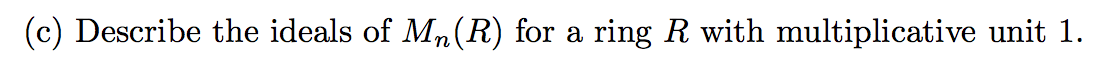
\includegraphics[width=350pt]{img/linear-algebra-a0-1-6-c.png}\\
\end{mdframed}

\subsection*{} % 7
\begin{mdframed}
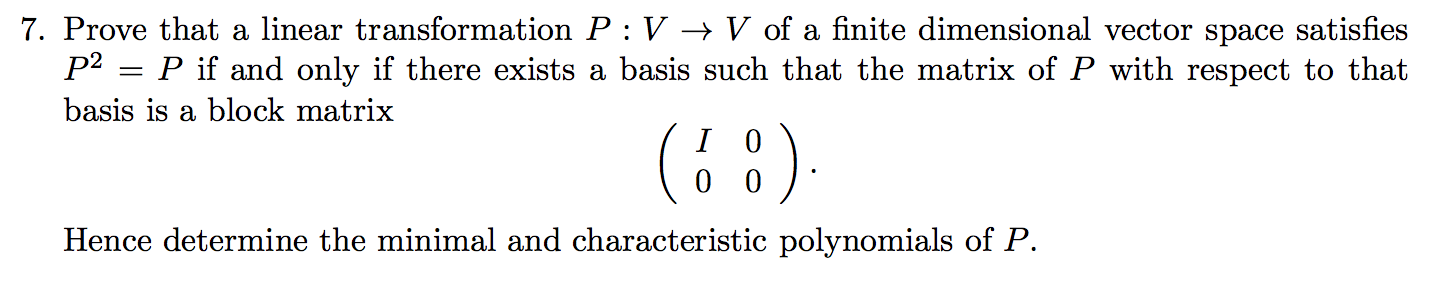
\includegraphics[width=400pt]{img/linear-algebra-a0-1-7.png}\\
\end{mdframed}

\subsection*{} % 8
\begin{mdframed}
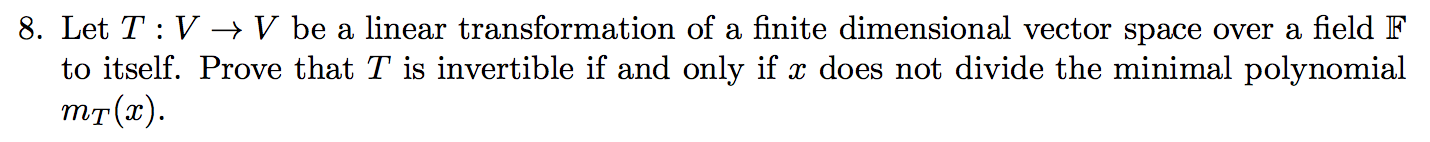
\includegraphics[width=400pt]{img/linear-algebra-a0-1-8.png}\\
\end{mdframed}

\subsection*{} % 9
\begin{mdframed}
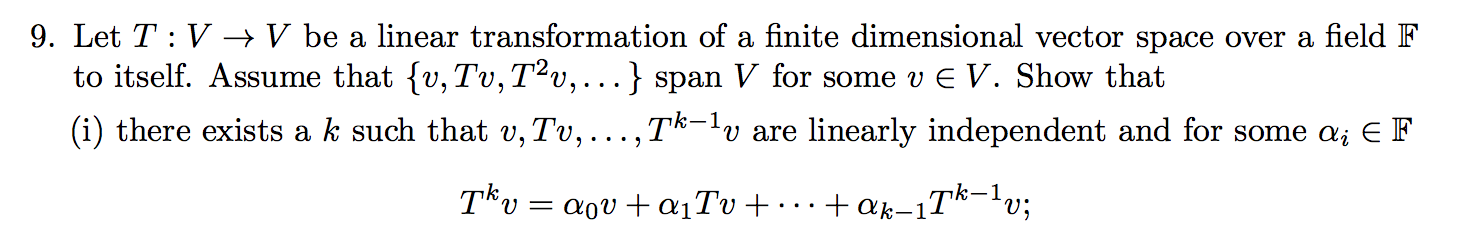
\includegraphics[width=400pt]{img/linear-algebra-a0-1-9-a.png}\\
\end{mdframed}
\begin{mdframed}
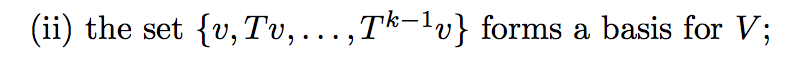
\includegraphics[width=280pt]{img/linear-algebra-a0-1-9-b.png}\\
\end{mdframed}
\begin{mdframed}
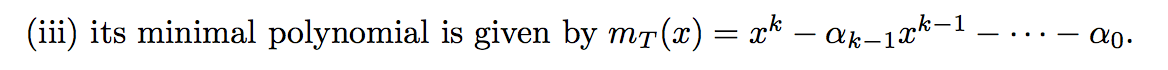
\includegraphics[width=400pt]{img/linear-algebra-a0-1-9-c.png}\\
\end{mdframed}
\begin{mdframed}
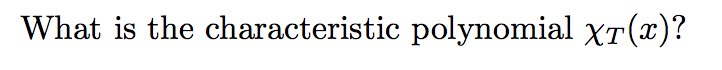
\includegraphics[width=270pt]{img/linear-algebra-a0-1-9-d.png}\\
\end{mdframed}

\end{document}
